\chapter[二维分数阶非线性Schr{\"o}dinger波方程的显式高阶保结构算法]{二维分数阶非线性Schr{\"o}dinger波方程的显式高阶保结构算法}

\section{NFSWE的SAV重构}\label{Section 2}
在本节中,我们回顾了开发高效节能方案来解决 NFSWE 的主要挑战在于非线性项的离散化.
正如我们所知,所有 RK 方法都保留任意线性不变量 \cite{griffithsNumericalMethodsOrdinary2010},辛 RK 方法保留任意二次不变量\cite{cooperStabilityRungeKuttaMethods1987}.
然而,没有 RK 方法可以保留任意多项式不变量的次数高于两个或非多项式非线性不变量 \cite{calvoNumericalSolutionIsospectral1997}.
在本节中,为了利用松弛 RK 方法的二次不变性保持特性,我们将采用新开发的标量辅助变量方法将高次能量重写为二次能量,
然后将 NFSWE 重新表述为允许二次能量函数的等效形式.

在介绍该方案之前,我们引入一个标量辅助变量 (SAV),即让
\begin{equation}
	w(t)=\sqrt{H(t)+C_0} \text { with } H(t)=\frac{\beta}{2}\|u(\cdot, t)\|_{L^{4}}^{4} .
\end{equation}
直接计算得出
\begin{equation}
	   \begin{aligned}
		w_t & =\frac{1}{2 \sqrt{H(t)+C_0}} \frac{d H(t)}{d t} \\
		& =\frac{1}{2 \sqrt{H(t)+C_0}} \frac{d}{d t} \int_{\Omega} \frac{\beta}{2}|u|^{4}d \boldsymbol{x} \\
		& =\frac{\beta}{\sqrt{H(t)+C_0}} \int_{\Omega} |u|^2 \Re\left(u \bar{u}_t\right) d \boldsymbol{x} \quad\left(\frac{d|u|^2}{d t}=2 \Re\left(u \bar{u}_t\right)\right) \\
		& =\Re \int_{\Omega} \frac{\beta|u|^2 u \bar{u}_t}{\sqrt{H(t)+C_0}} d \boldsymbol{x} \\
		& =\Re\left(b(u), u_t\right) \quad\left(b(u)=\beta|u|^2 u / \sqrt{H(t)+C_0}\right)
		\end{aligned}\label{eq:2-1}
\end{equation}
其中 $\Re(\cdot)$ 表示取复数的实部,$(\cdot, \cdot)$ 表示对 $\Omega$ 的 $L^2$ 内积.因此,模型问题 \eqref{eq:s1} 可以等价地改写为
\begin{align}
& u_t=v, \label{eq:2-2}\\
& v_t=-(-\Delta)^{\alpha / 2} u-\mathrm{i}\kappa v-b(u) w, \label{eq:2-3}\\
& w_t=\Re\left(b(u), u_t\right) .\label{eq:2-4}
\end{align}

与初始条件
\begin{align}\label{eq_31}
u(\boldsymbol{x}, 0)=u_{0}(\boldsymbol{x}), \quad v(\boldsymbol{x}, 0)=u_{1}(\boldsymbol{x}), \quad w(0)=\sqrt{\frac{\beta}{2}\|u(\cdot, 0)\|_{L^{4}}^{4} +C_0}.
\end{align}

对系统 \eqref{eq:2-2}-\eqref{eq:2-3} 分别取 $v_t$ 和 $u_t$ 的内积,将 \eqref{eq:2-4} 乘以 $w(t )$,对得到的方程求和,最后在时间间隔 $[0, t]$ 上对实部进行积分,立即得到修改后的能量守恒定律
\begin{equation}
E(t)=\|v(\cdot, t)\|^2+\left\|(-\Delta)^{\frac{\alpha}{4}} u(\cdot, t)\right\|^{2}+w^2(t)=E(0)
\end{equation}
这对应于具有周期边界的问题 \eqref{eq:s1} 的原始能量守恒定律 \eqref{eq_9}.
\section{保结构空间离散化}\label{Section 3}

% \subsection{Space Semi-discrete System}
注意到周期性边界条件,我们选择傅立叶伪谱方法对 NFSWEs \eqref{eq:2-2}-\eqref{eq_31} 进行空间离散化.%We develop a numerical method to solve the initial-periodic boundary value problem \eqref{eq:s1} in a finite domain $\Omega \times(0, T)$.

不失一般性,我们设置$d=2$.
%First, we introduce some notations.
对于正整数$M$甚至正整数$N_{x}$和$N_{y}$,表示$\tau={T}/{M},h_{x}={2 L}/{N_{ x}}, h_{y}={2 L}/{N_{y}}$.定义 $\Omega_{h}^{\tau}=\Omega_{h} \times \Omega_{\tau}$,其中 $\Omega_{h}=\left\{\left(x_{i}, y_{ j}\right) \mid i=0,1, \cdots, N_{x}\!-\!1;\right.\\ \left.j=0,1, \cdots, N_{y}\! -\!1\right\}$ 和 $\Omega_{\tau}=\left\{t_{m} \mid t_{m}=m \tau, 0 \leq m \leq M\right\}$,其中 $t_{m}=m \tau, x_{i}\!=\!-L i h_{x}$ 和 $y_{j}\!=\!-L j h_{y}$.
然后给出任何时间级别的相应向量形式
\begin{align}\label{eq_47}
&U^m=\left(u_{0,0}^m, \cdots, u_{N_{x}-1,0}^m, u_{0,1}^m, \cdots, u_{N_{x}-1,1}^m, \cdots, u_{0, N_{y}-1}^m, \cdots, u_{N_{x}-1, N_{y}-1}^m\right)^{T}.\\
&V^m=\left(v_{0,0}^m, \cdots, v_{N_{x}-1,0}^m, v_{0,1}^m, \cdots, v_{N_{x}-1,1}^m, \cdots, v_{0, N_{y}-1}^m, \cdots, v_{N_{x}-1, N_{y}-1}^m\right)^{T}.\\
&W^m=w^m.
\end{align}
对于任何网格函数 $u,v\in \Omega_{h}^{\tau}$,
将离散内积和相关的离散范数定义为
\begin{align}\label{eq_48}
(u, v)=h_{x} h_{y} \sum_{i=0}^{N_{x}-1} \sum_{j=0}^{N_{y}-1} u_{i, j} \bar{v}_{i, j}, \quad\|u\|=(u, u)^{\frac{1}{2}}, \quad\|u\|_{\infty}=\sup _{\left(x_{i}, y_{j}\right) \in \Omega_{h}}\left|u_{i, j}\right|.
\end{align}

令 $\left(x_{i}, y_{j}\right) \in \Omega_{h}$ 为傅里叶配置点.表示 $u_{N}(x, y)$ 是
$u(x, y)$ 的插值多项​​式函数,那么我们有
\begin{align}\label{eq_50}
u_{N}(x, y)=\sum_{k_{1}=-N_{x} / 2}^{N_{x} / 2} \sum_{k_{2}=-N_{y} / 2}^{N_{y} / 2} \tilde{u}_{k_{1}, k_{2}} e^{\mathrm{i}\mu\left( k_{1} (x+L)+k_{2}(y+L)\right)},
\end{align}
其中$\mu={\pi}/{L}$,以及系数
\begin{align}\label{eq_51}
\tilde{u}_{k_{1}, k_{2}}=\frac{1}{N_{x} c_{k_{1}}} \frac{1}{N_{y} c_{k_{2}}} \sum_{l_1=0}^{N_{x}-1} \sum_{l_2=0}^{N_{y}-1} u(x_{l_1}, y_{l_2}) e^{-\mathrm{i}\mu\left( k_{1}(x_{l_1}+L)+k_{2}(y_{l_2}+L)\right)},
\end{align}
其中 $c_{k_{1}}=1$ 对于 $\left|k_{1}\right|<N_{x} / 2, c_{k_{2}}=1$ 对于 $\left|k_{2 }\right|<N_{y} / 2, c_{k_{1}}=2$ 对于 $k_{1}=\pm N_{x} / 2$, $c_{k_{2}}=2$对于$ k_{2}=\pm N_{y} / 2$.
因此,分数拉普拉斯算子 $-(-\Delta)^{\frac{\alpha}{2}} u(x, y)$ 可以近似为
\begin{align}\label{eq_52}
-(-\Delta)^{\frac{\alpha}{2}} u_{N}\left(x, y\right)=-\sum\limits_{k_{1}=-N_{x} / 2}^{N_{x} / 2} \sum\limits_{k_{2}=-N_{y} / 2}^{N_{y} / 2}\left|\left(k_{1} \mu\right)^{2}+\left(k_{2} \mu\right)^{2}\right|^{\frac{\alpha}{2}} \tilde{u}_{k_{1}, k_{2}} e^{\mathrm{i}\mu\left( k_{1} (x+L)+k_{2}(y+L)\right)},
\end{align}
% where $\sum\limits_{\mathbf{k}=-\mathbf{N} / 2}^{\mathbf{N} / 2}=\sum\limits_{k_{1}=-N_{x} / 2}^{N_{x} / 2} \sum\limits_{k_{2}=-N_{y} / 2}^{N_{y} / 2}, \mathbf{k} \cdot(\boldsymbol{x}+\mathbf{L})=k_{1}(x+L)+k_{2}(y+L)$.
%We denote $u_{i, j}=u\left(x_{i}, y_{j}\right), \mu^{2} \cdot \mathbf{k}^{2}=\mu^{2}\left(k_{1}^{2}+k_{2}^{2}\right)$ and
将 \eqref{eq_51} 插入 \eqref{eq_52},并考虑点 $(x_i,y_j)$ 处的结果方程给出
\begin{align}
&-(-\Delta)^{\frac{\alpha}{2}} u_{N}\left(x_{i}, y_{j}\right)\nonumber\\
%=&-\sum\limits_{k_{1}=-N_{x} / 2}^{N_{x} / 2} \sum\limits_{k_{2}=-N_{y} / 2}^{N_{y} / 2}\left|\mu^{2} \cdot \mathbf{k}^{2}\right|^{\frac{\alpha}{2}}\left(\frac{1}{N_{x} %c_{k_{1}}} \frac{1}{N_{y} c_{k_{2}}} \sum\limits_{l_{1}=0}^{N_{x}-1} \sum\limits_{l_{2}=0}^{N_{y}-1}u_{l_{1}, l_{2}} e^{-\mathrm{i}\mu\left( %k_{1}(x_{l_1}+L)+k_{2}(y_{l_2}+L)\right)}\right) e^{\mathrm{i} \mu\left(k_{1}\left(x_{i}+L\right)+k_{2}\left(y_{j}+L\right)\right)}\nonumber\\
=&\sum\limits_{l_{1}=0}^{N_{x}-1} \sum\limits_{l_{2}=0}^{N_{y}-1}u(x_{l_{1}}, y_{l_{2}})\left(-\sum\limits_{k_{1}=-N_{x} / 2}^{N_{x} / 2} \sum\limits_{k_{2}=-N_{y} / 2}^{N_{y} / 2} \frac{1}{N_{x} c_{k_{1}}} \frac{1}{N_{y} c_{k_{2}}}\left|\mu^{2} \cdot \mathbf{k}^{2}\right|^{\frac{\alpha}{2}} e^{\mathrm{i} \mu\left(k_{1}\left(x_{i}-x_{l_{1}}\right)+k_{2}\left(y_{j}-y_{l_{2}}\right)\right)}\right)\nonumber\\
=&\left(D^{\alpha}U\right)_{i+j N_{x}},\label{eq_53}
\end{align}
% where $\mu^{2} \cdot \mathbf{k}^{2}=\mu^{2}\left(k_{1}^{2}+k_{2}^{2}\right), \boldsymbol{x_l}+\mathbf{L}=\left(x_{l_{1}}+L\right)+\left(y_{l_{2}}+L\right)$,
其中 $\mu^{2} \cdot \mathbf{k}^{2}=\mu^{2}\left(k_{1}^{2} k_{2}^{2}\right)$, $D^{\alpha}$ 是具有元素的谱对称微分矩阵
\begin{align}\label{eq_54}
\left(D^{\alpha}\right)_{i+j N_{x}, l_{1}+l_{2} N_{x}}=-\sum\limits_{l_{1}=0}^{N_{x}-1} \sum\limits_{l_{2}=0}^{N_{y}-1}\frac{1}{N_{x} c_{k_{1}}} \frac{1}{N_{y} c_{k_{2}}}\left|\mu^{2} \cdot \mathbf{k}^{2}\right|^{\frac{\alpha}{2}} e^{\mathrm{i}\mu\left(k_{1}\left(x_{i}-x_{l_{1}}\right)+k_{2}\left(y_{j}-y_{l_{2}}\right)\right)}.
\end{align}


%\begin{remark}
%	\label{rmk1}
%	The spectral differential matrix $D^{\alpha}$ is a symmetric matrix with the elements
%\begin{align}\label{eq_54}
%\left(D^{\alpha}\right)_{i+j N_{x}, l_{1}+l_{2} N_{x}}=-\sum_{\mathbf{k}=-\mathbf{N} / 2}^{\mathbf{N} / 2} \frac{1}{N_{x} c_{k_{1}}} \frac{1}{N_{y} c_{k_{2}}}\left|\mu^{2} \cdot \mathbf{k}^{2}\right|^{\frac{\alpha}{2}} e^{-i \mu\left(k_{1}\left(x_{i}-x_{l_{1}}\right)+k_{2}\left(y_{j}-y_{l_{2}}\right)\right)}.
%\end{align}
%\end{remark}

% \begin{pf}
	
% \begin{equation}
% 	\begin{aligned}
% 	\left(D^{S}\right)_{i+j N_{x}, l_{1}+l_{2} N_{x}} &=-\sum_{\mathbf{k}=-\mathbf{N} / 2}^{\mathbf{N} / 2} \frac{1}{N_{x} c_{k_{1}}} \frac{1}{N_{y} c_{k_{2}}}\left|\mu^{2} \cdot \mathbf{k}^{2}\right|^{\frac{\alpha}{2}} e^{-\mathrm{i} \mu\left(k_{1}\left(x_{i}-x_{l_{1}}\right)+k_{2}\left(y_{j}-y_{l_{2}}\right)\right)} \\
% 	&=-\sum_{\mathbf{k}=-\mathbf{N} / 2}^{\mathbf{N} / 2} \frac{1}{N_{x} c_{k_{1}}} \frac{1}{N_{y} c_{k_{2}}}\left|\mu^{2} \cdot(-\mathbf{k})^{2}\right|^{\frac{\alpha}{2}} e^{-\mathrm{i} \mu\left(\left(-k_{1}\right)\left(x_{l_{1}}-x_{i}\right)+\left(-k_{2}\right)\left(y_{l_{2}}-y_{j}\right)\right)} \\
% 	&=-\sum_{\mathbf{k}=-\mathbf{N} / 2}^{\mathbf{N} / 2} \frac{1}{N_{x} c_{k_{1}}} \frac{1}{N_{y} c_{k_{2}}}\left|\mu^{2} \cdot \mathbf{k}^{2}\right|^{\frac{\alpha}{2}} e^{-\mathrm{i} \mu\left(k_{1}\left(x_{l_{1}}-x_{i}\right)+k_{2}\left(y_{l_{2}}-y_{j}\right)\right)} \\
% 	&=\left(D^{S}\right)_{l_{1}+l_{2} N_{x}, i+j N_{x}}
% 	\end{aligned}
% 	\label{eq_55}\end{equation}
% 	where we have used the fact that $c_{k_{1}}=1$ for $\left|k_{1}\right|<N_{x} / 2, c_{k_{2}}=1$ for $\left|k_{2}\right|<N_{y} / 2, c_{k_{1}}=2$ for $k_{1}=\pm N_{x} / 2$, and $c_{k_{1}}=2$ for $k_{2}=\pm N_{y} / 2 .$ The proof is complete.
% \end{pf}

应用傅里叶伪谱法逼近前面空间中的等效系统\eqref{eq:2-2}-\eqref{eq:2-4},得到空间半离散系统如下
\begin{align}
	& U_t=V, \label{eq:3-9}\\
	& V_t=D^{\alpha} U-\mathrm{i}\kappa V- b(U) \cdot W, \label{eq:3-10}\\
	& W_t=\Re\left(b(U), U_t\right) .\label{eq:3-11}
	\end{align}

	具有初始条件 $U^0, V^0, W^0$,其中 $\cdot$ 表示向量之间的点乘.那么我们有下面的定理.
    \begin{thm}	\label{thm3}
        半离散系统\eqref{eq:3-9}–\eqref{eq:3-11}承认半离散全局二次能量守恒定律
        % 	\begin{equation}
% 		E(U,V,W):=\|V\|^2 - \left(U, D^{\alpha} U\right)+\left(W\right)^2 \equiv \text { Const. }
% 		\end{equation}
\begin{equation}
	E(U,V,W):=\|V\|^2 + \|D^\frac{\alpha}{2} U\|^2+\left(W\right)^2 \equiv \text { Const. }\label{eq:313}
	\end{equation}
\end{thm}

\begin{pf}
    对系统 \eqref{eq:3-9}-\eqref{eq:3-10} 分别取 $V_t$ 和 $U_t$ 的内积,
    将 \eqref{eq:3-11} 乘以 $W$,
\begin{align}
	  \left(V_t, U_t\right)&=\left(V_t, V\right), \\
	 \left(V_t, U_t\right)&=\left(D^{\alpha} U, U_t\right)-i \kappa\left(V, U_t\right)-W\left(b(U), U_t\right), \\
	 W W_t&=W\Re\left(b(U), U_t\right),
	\end{align}
    对得到的方程求和
\begin{equation}
	\left(V_t, V\right) + W W_t= \left(D^{\alpha} U, U_t\right)-i \kappa\left(V, U_t\right)-W\left(b(U), U_t\right) + W\Re\left(b(U), U_t\right),
\end{equation}
并取实部得到
\begin{align}
	\Re\left(V_t, V\right) + \Re\left(W W_t\right)&= \Re\left(D^{\alpha} U, U_t\right)-\Re\left(i \kappa\left(V, U_t\right)\right)-W\Re\left(b(U), U_t\right) + W\Re\left(b(U), U_t\right),\\
	\Re\left(V_t, V\right) + \Re\left(W W_t\right)&= \Re\left(D^{\alpha} U, U_t\right).\label{eq:319}
\end{align}
很容易验证
\begin{equation}
	\Re\left(V_t, V\right) = \frac{1}{2}\frac{d }{d t}\|V\|^2, \quad \Re\left(W W_t\right) = \frac{1}{2}\frac{d }{d t}\left(W\right)^2,\quad \Re\left(D^{\alpha} U, U_t\right)=-\frac{1}{2}\frac{d }{d t}\|D^\frac{\alpha}{2}U\|^2\label{eq:320}
\end{equation}
将方程\eqref{eq:320}代入方程\eqref{eq:319},可以得到
\begin{equation}
	\frac{d }{d t}\left(\|V\|^2+\left(W\right)^2+\|D^\frac{\alpha}{2}U\|^2\right)=0.
\end{equation}
这意味着方程\eqref{eq:313}
\end{pf}
\section{守恒SAV-RRK格式}\label{Section 4}
为了加速计算,因此,我们采用SAV方法为NFSWEs提出了不变量保持的显式Runge-Kutta方案.本节开始,我们回顾RRK方法并讨论它们的结构保持特性.
\subsection{Explicit SAV-RRK schemes}
为简洁起见,我们引入以下符号:
\begin{equation}
	\bm{y}=\left(U,V,W\right)^T,\bm{y}_0=\left(U^0,V^0,W^0\right)^T , \bm{f}=(f^1,f^2,f^3)^T=(V,D^{\alpha} U-\mathrm{i}\kappa V-b(U)\cdot W,\Re\left(b(U), U_t\right))^T.
\end{equation}
然后,NFSWEs\eqref{eq:3-9}-\eqref{eq:3-11} 可以重写为:
\begin{equation}
	\left\{\begin{array}{l}
	\bm{y}_t=\bm{f}(\bm{y}),\quad t \in(0, T]\\
	\bm{y}(0)=\bm{y}_0.
\end{array}\right.\label{eq:3-121}
\end{equation}
设 $\bm{y}^m$ 和 $\bm{y}^{m+1}$ 分别为 $\bm{y}\left(t_m\right)$ 和 $\bm{y}\left(t_{m+1}\right)$ 的数值逼近;应用于式 \eqref{eq:3-121} 的 $s$ 阶显式 SAV-RK 方法的形式如下:
\begin{equation}
	\left\{\begin{array}{l}
		\bm{Y}_{m i}=\bm{y}^m+\tau \sum\limits_{j=1}^i a_{i j} \bm{f}_{m j}, \quad i=1, \ldots, s, \\
		\bm{y}^{m+1}=\bm{y}^m+\tau \sum\limits_{i=1}^s b_i \bm{f}_{m i}
	\end{array}\right.\label{eq:4-31}
	\end{equation}
    其中 $m=0, \ldots, M-1$,$\bm{f}{m j}=\bm{f}\left(\bm{Y}{m j}\right)$,$j=1, \ldots, s$.以下是相关符号的定义:
\begin{equation}
\begin{aligned}
A & =\left(a_{i j}\right)_{s \times s}, \quad a_{i j}=0 \quad \text { for } \quad j \geq i, \\
b & =\left(b_1, \cdots, b_s\right)^T,
\end{aligned}
\end{equation}
$s$ 阶 SAV-RK 方法可以用Butcher阵列表示,如下所示:
\begin{equation}
	\begin{array}{c|c}
	c & A \\
	\hline \\
	& b^T
	\end{array}
	\end{equation}
    其中,横坐标向量 $c$ 满足 $c_i=\sum\limits_{j=1}^s a_{i j}, i=1, \ldots, s$.

    然而,众所周知,某些隐式 RK 方法可能是辛型的或代数稳定的,但是没有一种显式 RK 方法是辛型的或代数稳定的.这导致 SAV-RK 方法无法保持守恒性质.
    
    考虑在区间 $\left[\hat{t}m, \hat{t}{m+1}\right], m \geq 0$ 上进行一步计算,设 $\bm{y}\gamma^m$ 和 $\bm{y}\gamma^{m+1}$ 分别是 $\bm{y}\left(\hat{t}m\right)$ 和 $\bm{y}\left(\hat{t}{m+1}\right)$ 的数值逼近,则式 \eqref{eq:3-121} 的 $s$ 阶显式 SAV-RRK 方法定义如下:
    \begin{equation}
	\left\{\begin{array}{l}
		\bm{Y}_{m i}=\bm{y}_\gamma^m+\tau \sum\limits_{j=1}^i a_{i j} \bm{f}_{m j}, \quad i=1, \ldots, s, \\
		\bm{y}_\gamma^{m+1}=\bm{y}_\gamma^m+\gamma_m \tau \sum\limits_{i=1}^s b_i \bm{f}_{m i}
	\end{array}\right.\label{eq:4-3}
	\end{equation}
% for $m=0, \ldots, M-1$, where $\bm{f}_{m j}=\bm{f}\left(\bm{Y}_{m j}\right)$, $j=1, \ldots, s$. With the following notations
% \begin{equation}
% \begin{aligned}
% A & =\left(a_{i j}\right)_{s \times s}, \quad a_{i j}=0 \quad \text { for } \quad j \geq i, \\
% b & =\left(b_1, \cdots, b_s\right)^T,
% \end{aligned}
% \end{equation}
$s$ 阶 SAV-RRK 方法可以用Butcher阵列表示,如下所示:
\begin{equation}
	\begin{array}{c|c}
	c & A \\
	\hline \\
	& \tilde{b}^T
	\end{array}
	\end{equation}
    其中,$\tilde{b}=\gamma_m b$,$\gamma_m\neq 0$ 满足以下条件:
\begin{equation}
	\left\{\begin{array}{ll}
	% E_{\gamma}^{m+1}=E_{\gamma}^{m}+2 \gamma_m \tau \sum\limits_{i=1}^s \Re\left\langle -\mathrm{i}\kappa V_{\gamma}^{m}+(1-\beta) b(U_{\gamma}^{m})\cdot W_{\gamma}^{m}, b_i \bm{f}_{m i}\right\rangle, &\text { if } \sum\limits_{i=1}^s b_i \bm{f}_{m i} \neq 0,\\
	E_{\gamma}^{m+1}=E_{\gamma}^{m}, &\text { if } \sum\limits_{i=1}^s b_i \bm{f}_{m i} \neq 0,\\
	\gamma_m=1, &\text { if } \sum\limits_{i=1}^s b_i \bm{f}_{m i} =0.
	\end{array}\right.\label{eq:4-6}
	\end{equation}
    在 $\hat{t}{m+1}$ 处,对数值解 $\bm{y}\gamma^{m+1}$ 可以有两种解释方式.

	\textbf{Incremental direction technique (IDT):} $\bm{y}_\gamma^{m+1}$ is viewed as the approximation to $\bm{y}\left(\hat{t}_m+\tau\right)$, then $\hat{t}_m=t_m, m \geq 0$.

	\textbf{Relaxation technique (RT):} $ \bm{y}_\gamma^{m+1}$ is viewed as the approximation to $\bm{y}\left(\hat{t}_m+\right.\left.\gamma_m \tau\right)$, then $\hat{t}_m$ may not be equal to $t_m$ when $m>0$.

需要指出的是,对数值解 $\bm{y}_\gamma^{m+1}$ 的不同理解将导致不同的收敛结果.

当且仅当 $\sum\limits_{i=1}^s b_i \bm{f}_{m i}\neq 0$ 时,$\gamma_m$ 的值也可以被明确地表达.经过简单的计算,我们可以得到:

% \begin{equation}
% 	\begin{aligned}
% 	 E_{\gamma}^{m+1}  =&\|V_{\gamma}^{m+1}\|^2- \left(U_{\gamma}^{m+1}, D^{\alpha} U_{\gamma}^{m+1}\right)+\left(W_{\gamma}^{m+1}\right)^2 \\
% 	 =&\|V_{\gamma}^{m}+\gamma_m\tau\sum\limits_{i=1}^{s}b_if_{mi}^2\|^2- \left(U_{\gamma}^{m}+\gamma_m\tau\sum\limits_{i=1}^{s}b_if_{mi}^1, D^{\alpha} \left(U_{\gamma}^{m}+\gamma_m\tau\sum\limits_{i=1}^{s}b_if_{mi}^1\right)\right)+\left(W_{\gamma}^{m}+\gamma_m\tau\sum\limits_{i=1}^{s}b_if_{mi}^3\right)^2\\
% 	 =&\|V_{\gamma}^{m}\|^2- \left(U_{\gamma}^{m}, D^{\alpha} U_{\gamma}^{m}\right)+\left(W_{\gamma}^{m}\right)^2\\
% 	 &+\left(V_{\gamma}^{m},\gamma_m\tau\sum\limits_{i=1}^{s}b_if_{mi}^2\right)+\left(\gamma_m\tau\sum\limits_{i=1}^{s}b_if_{mi}^2,V_{\gamma}^{m}\right)+\left(\gamma_m\tau\sum\limits_{i=1}^{s}b_if_{mi}^2,\gamma_m\tau\sum\limits_{i=1}^{s}b_if_{mi}^2\right)\\
% 	 &- \left(U_{\gamma}^{m}, D^{\alpha} \left(\gamma_m\tau\sum\limits_{i=1}^{s}b_if_{mi}^1\right)\right)- \left(\gamma_m\tau\sum\limits_{i=1}^{s}b_if_{mi}^1, D^{\alpha}U_{\gamma}^{m}\right)\\
% 	 &- \left(\gamma_m\tau\sum\limits_{i=1}^{s}b_if_{mi}^1, D^{\alpha}\left(\gamma_m\tau\sum\limits_{i=1}^{s}b_if_{mi}^1\right)\right)+2W_{\gamma}^{m}\gamma_m\tau\sum\limits_{i=1}^{s}b_if_{mi}^3+\left(\gamma_m\tau\sum\limits_{i=1}^{s}b_if_{mi}^3\right)^2\\
% 	=& E_{\gamma}^{m}+\gamma_m\tau\left[\left(V_{\gamma}^{m},\sum\limits_{i=1}^{s}b_if_{mi}^2\right)+\left(\sum\limits_{i=1}^{s}b_if_{mi}^2,V_{\gamma}^{m}\right)\right.\\
% 	&\left.-\left(U_{\gamma}^{m},D^{\alpha} \left(\sum\limits_{i=1}^{s}b_if_{mi}^1\right)\right)-\left(\sum\limits_{i=1}^{s}b_if_{mi}^1, D^{\alpha} U_{\gamma}^{m}\right)+2W_{\gamma}^{m}\sum\limits_{i=1}^{s}b_if_{mi}^3\right]\\
% 	 &+\gamma_m^2\tau^2\left[\left(\sum\limits_{i=1}^{s}b_if_{mi}^2,\sum\limits_{i=1}^{s}b_if_{mi}^2\right)- \left(\sum\limits_{i=1}^{s}b_if_{mi}^1,D^{\alpha}\left(\sum\limits_{i=1}^{s}b_if_{mi}^1\right)\right)+\left(\sum\limits_{i=1}^{s}b_if_{mi}^3\right)^2\right].
% 	\end{aligned}
% 	\end{equation}
\begin{equation}
	\begin{aligned}
	 E_{\gamma}^{m+1}  =&\|V_{\gamma}^{m+1}\|^2+\|D^\frac{\alpha}{2} U_{\gamma}^{m+1}\|^2+\left(W_{\gamma}^{m+1}\right)^2 \\
	 =&\|V_{\gamma}^{m+1}\|^2- \left(U_{\gamma}^{m+1}, D^{\alpha} U_{\gamma}^{m+1}\right)+\left(W_{\gamma}^{m+1}\right)^2 \\
	 =&\|V_{\gamma}^{m}+\gamma_m\tau\sum\limits_{i=1}^{s}b_if_{mi}^2\|^2- \left(U_{\gamma}^{m}+\gamma_m\tau\sum\limits_{i=1}^{s}b_if_{mi}^1, D^{\alpha} \left(U_{\gamma}^{m}+\gamma_m\tau\sum\limits_{i=1}^{s}b_if_{mi}^1\right)\right)+\left(W_{\gamma}^{m}+\gamma_m\tau\sum\limits_{i=1}^{s}b_if_{mi}^3\right)^2\\
	 =&\|V_{\gamma}^{m}\|^2+\|D^\frac{\alpha}{2} U_{\gamma}^{m}\|^2+\left(W_{\gamma}^{m}\right)^2\\
	 &+\left(V_{\gamma}^{m},\gamma_m\tau\sum\limits_{i=1}^{s}b_if_{mi}^2\right)+\left(\gamma_m\tau\sum\limits_{i=1}^{s}b_if_{mi}^2,V_{\gamma}^{m}\right)+\left\|\gamma_m\tau\sum\limits_{i=1}^{s}b_if_{mi}^2\right\|^2\\
	 &- \left(U_{\gamma}^{m}, D^{\alpha} \left(\gamma_m\tau\sum\limits_{i=1}^{s}b_if_{mi}^1\right)\right)- \left(\gamma_m\tau\sum\limits_{i=1}^{s}b_if_{mi}^1, D^{\alpha}U_{\gamma}^{m}\right)\\
	 &+ \left\|D^\frac{\alpha}{2}\left(\gamma_m\tau\sum\limits_{i=1}^{s}b_if_{mi}^1\right)\right\|^2+2W_{\gamma}^{m}\gamma_m\tau\sum\limits_{i=1}^{s}b_if_{mi}^3+\left(\gamma_m\tau\sum\limits_{i=1}^{s}b_if_{mi}^3\right)^2\\
	=& E_{\gamma}^{m}+\gamma_m\tau\left[\left(V_{\gamma}^{m},\sum\limits_{i=1}^{s}b_if_{mi}^2\right)+\left(\sum\limits_{i=1}^{s}b_if_{mi}^2,V_{\gamma}^{m}\right)\right.\\
	&\left.-\left(U_{\gamma}^{m},D^{\alpha} \left(\sum\limits_{i=1}^{s}b_if_{mi}^1\right)\right)-\left(\sum\limits_{i=1}^{s}b_if_{mi}^1, D^{\alpha} U_{\gamma}^{m}\right)+2W_{\gamma}^{m}\sum\limits_{i=1}^{s}b_if_{mi}^3\right]\\
	 &+\gamma_m^2\tau^2\left[\left\|\sum\limits_{i=1}^{s}b_if_{mi}^2\right\|^2+ \left\|D^\frac{\alpha}{2}\left(\sum\limits_{i=1}^{s}b_if_{mi}^1\right)\right\|^2+\left(\sum\limits_{i=1}^{s}b_if_{mi}^3\right)^2\right].
	\end{aligned}\label{eq:49}
	\end{equation}
    这个式子和 \eqref{eq:4-6} 结合起来,得到:
\begin{equation}
\begin{aligned}
	&\gamma_m\tau\left[\left(V_{\gamma}^{m},\sum\limits_{i=1}^{s}b_if_{mi}^2\right)+\left(\sum\limits_{i=1}^{s}b_if_{mi}^2,V_{\gamma}^{m}\right)-\left(U_{\gamma}^{m},D^{\alpha} \left(\sum\limits_{i=1}^{s}b_if_{mi}^1\right)\right)-\left(\sum\limits_{i=1}^{s}b_if_{mi}^1, D^{\alpha} U_{\gamma}^{m}\right)+2W_{\gamma}^{m}\sum\limits_{i=1}^{s}b_if_{mi}^3\right]\\
	 &+\gamma_m^2\tau^2\left[\left\|\sum\limits_{i=1}^{s}b_if_{mi}^2\right\|^2+ \left\|D^\frac{\alpha}{2}\left(\sum\limits_{i=1}^{s}b_if_{mi}^1\right)\right\|^2+\left(\sum\limits_{i=1}^{s}b_if_{mi}^3\right)^2\right]=0,
	\end{aligned}
\end{equation}
注意到 $\gamma_m \neq 0$,所以可以得到:
\begin{equation}
	\gamma_m=-\frac{\left(V_{\gamma}^{m},\sum\limits_{i=1}^{s}b_if_{mi}^2\right)+\left(\sum\limits_{i=1}^{s}b_if_{mi}^2,V_{\gamma}^{m}\right)-\left(U_{\gamma}^{m},D^{\alpha} \left(\sum\limits_{i=1}^{s}b_if_{mi}^1\right)\right)-\left(\sum\limits_{i=1}^{s}b_if_{mi}^1, D^{\alpha} U_{\gamma}^{m}\right)+2W_{\gamma}^{m}\sum\limits_{i=1}^{s}b_if_{mi}^3}{\tau\left[\left\|\sum\limits_{i=1}^{s}b_if_{mi}^2\right\|^2+ \left\|D^\frac{\alpha}{2}\left(\sum\limits_{i=1}^{s}b_if_{mi}^1\right)\right\|^2+\left(\sum\limits_{i=1}^{s}b_if_{mi}^3\right)^2\right]} .
% \gamma_m=\frac{\left(V_{\gamma}^{m}\right)^T \left(\sum\limits_{i=1}^{s}b_if_{mi}^2\right)+\left(\sum\limits_{i=1}^{s}b_if_{mi}^2\right)^T \left(V_{\gamma}^{m}\right)-\left(U_{\gamma}^{m}\right)^T D^{\alpha} \left(\sum\limits_{i=1}^{s}b_if_{mi}^1\right)-\left(\sum\limits_{i=1}^{s}b_if_{mi}^1\right)^T D^{\alpha} \left(U_{\gamma}^{m}\right)+2W_{\gamma}^{m}\sum\limits_{i=1}^{s}b_if_{mi}^3}{\tau\left[\left(\sum\limits_{i=1}^{s}b_if_{mi}^2\right)^T \left(\sum\limits_{i=1}^{s}b_if_{mi}^2\right)- \left(\sum\limits_{i=1}^{s}b_if_{mi}^1\right)^T D^{\alpha}\left(\sum\limits_{i=1}^{s}b_if_{mi}^1\right)+\left(\sum\limits_{i=1}^{s}b_if_{mi}^3\right)^2\right]} .
\end{equation}
由于$\bm{y}_\gamma^{m+1}$可以被视为对$\bm{y}\left(\hat{t}_m+\gamma_m \tau\right)$的逼近,因此在每一步中确保$\gamma_m>0$非常重要.事实上,\eqref{eq:4-6}中定义的$\gamma_m$对于小的步长$\tau$接近于$1$,这将在第\ref{Section 5-1}节进一步讨论.因此,松弛方法是良好定义的.

% \subsection{Structure-preserving properties of the RRK methods}
在公式 \eqref{eq:4-3} 中引入松弛系数 $\gamma_m$ 的目的是为了保证数值解的能量守恒.实验证明,SAV-RRK 方法对于保守问题 \eqref{eq:2-2}-\eqref{eq:2-4} 是保守的.
\begin{thm}
	假设 SAV-RK 方法 \eqref{eq:4-31} 至少为二阶方法;则对于足够小的步长 $\tau$,SAV-RRK 方法具有守恒性质
    \begin{equation}
	E_{\gamma}^{m+1}=E_{\gamma}^{m}\label{eq:4-10}
\end{equation}
这种守恒性质适用于保守问题.
\end{thm}

\begin{pf}
    当 $\sum_{i=1}^s b_i \bm{f}{m i}=0$ 时,根据 \eqref{eq:4-3} 中的第二个关系式可得 $\bm{y}\gamma^{m+1}=\bm{y}_\gamma^m$,从而自动满足性质 \eqref{eq:4-10}.

    当 $\sum_{i=1}^s b_i \bm{f}_{m i}\neq 0$ 时,根据条件 \eqref{eq:4-6},性质 \eqref{eq:4-10} 仍然成立.

由于 SAV-RK 方法的阶数至少为二,我们可以得出结论,在足够小的步长 $\tau$ 下,$\gamma_m>0$,这将在第 \ref{Section 5-1} 节中得到证明.
\end{pf}

\section{SAV-RRK 方法的精度}\label{Section 5}
本节中,我们将讨论 SAV-RRK 方法的精度.首先,我们估计松弛系数 $\gamma_m$,该系数在后续的分析中起着关键作用.然后,我们推导 SAV-RRK 方法的精度.

\subsection{松弛系数的估计}\label{Section 5-1}

虽然松弛系数 $\gamma_m$ 往往会随着步数而变化,但是它在不同步数间可以通过类似的方式进行估计.在这里,我们只考虑区间 $\left[\hat{t}m, \hat{t}{m+1}\right]$ 内的单个步长.在此期间,$\sum_{i=1}^s b_i \bm{f}{m i}=0$ 的情况较为简单,因此我们将重点放在 $\sum{i=1}^s b_i \bm{f}_{m i} \neq 0$ 的情况下.

设
% \begin{equation}
% 	S_m(\gamma)=\|V_\gamma^{m+1}\|^2 + \|D^\frac{\alpha}{2} U_\gamma^{m+1}\|^2+\left(W_\gamma^{m+1}\right)^2-\|V_\gamma^{m}\|^2 - \|D^\frac{\alpha}{2} U_\gamma^{m}\|^2-\left(W_\gamma^{m}\right)^2,
% \end{equation}
\begin{equation}
	\begin{aligned}
		S_m(\gamma)=&\left\|V_\gamma^m+\gamma \tau \sum\limits_{i=1}^s b_i \bm{f}_{m i}^2\right\|^2 + \left\|D^\frac{\alpha}{2} \left(U_\gamma^m+\gamma \tau \sum\limits_{i=1}^s b_i \bm{f}_{m i}^1\right)\right\|^2\\
	&+\left(W_\gamma^m+\gamma \tau \sum\limits_{i=1}^s b_i \bm{f}_{m i}^3\right)^2-\|V_\gamma^{m}\|^2 - \|D^\frac{\alpha}{2} U_\gamma^{m}\|^2-\left(W_\gamma^{m}\right)^2,
	\end{aligned}
	\end{equation}
    则,由 \eqref{eq:4-6} 定义的 $\gamma_m$ 的值恰为函数 $S_m(\gamma)$ 的非零根.对于 $S_m(\gamma)$,我们有引理 \ref{lem:5_1} 和引理 \ref{lem:5_2}.

\begin{lem}\label{lem:5_1}
	假设 SAV-RK 方法 \eqref{eq:4-31} 的阶数为 $p$,则对于足够小的 $\tau$,有以下结果成立:
    \begin{equation}
S_m(1)=\mathcal{O}\left(\tau^{p+1}\right)
\end{equation}
\end{lem} 
\begin{pf}
	考虑以下初值问题:
\begin{equation}
\left\{\begin{array}{l}
\tilde{\bm{y}}^{\prime}=\bm{f}(\tilde{\bm{y}}), \quad t \geq \hat{t}_m, \\
\tilde{\bm{y}}\left(\hat{t}_m\right)=\bm{y}_\gamma^m,
\end{array}\right.
\end{equation}
其中,$\bm{y}\gamma^m$与式\eqref{eq:4-3}中的相同.通过使用式\eqref{eq:4-31}中$p$阶的SAV-RK方法进行一步计算,我们可以得到内部阶段$\tilde{Y}{m i}, i=1, \ldots, s$以及数值解$\tilde{\bm{y}}^{m+1}$,其满足当$\tau$足够小时,$\tilde{\bm{y}}^{m+1}=\tilde{\bm{y}}\left(\hat{t}m+\tau\right)+\mathcal{O}\left(\tau^{p+1}\right)$.利用$\bm{y}\gamma^m$,带$\gamma_m=1$的SAV-RRK方法\eqref{eq:4-3}生成内部阶段$Y_{m i}, i=1, \ldots, s$和数值解$\bm{y}\gamma^{m+1}$.显然,$Y{m i}=\tilde{Y}{m i}, i=1, \ldots, s$,$\bm{y}\gamma^{m+1}=\tilde{\bm{y}}^{m+1}$.因此,令$\tilde{\bm{f}}{m i}:=\bm{f}\left(\tilde{Y}{m i}\right)$,我们有:
\begin{equation}
\begin{aligned}
S_n(1) = &\|V_\gamma^{m+1}\|^2 + \|D^\frac{\alpha}{2} U_\gamma^{m+1}\|^2+\left(W_\gamma^{m+1}\right)^2-\|V_\gamma^{m}\|^2 - \|D^\frac{\alpha}{2} U_\gamma^{m}\|^2-\left(W_\gamma^{m}\right)^2 \\
= &\|\tilde{V}^{m+1}\|^2 + \|D^\frac{\alpha}{2} \tilde{U}^{m+1}\|^2+\left(\tilde{W}^{m+1}\right)^2-\|\tilde{V}(\hat{t}_{m})\|^2 - \|D^\frac{\alpha}{2} \tilde{U}(\hat{t}_{m})\|^2-\left(\tilde{W}(\hat{t}_{m})\right)^2 \\
= &\|\tilde{V}^{m+1}\|^2 -\|\tilde{V}(\hat{t}_{m}+\tau)\|^2 +\|\tilde{V}(\hat{t}_{m}+\tau)\|^2-\|\tilde{V}(\hat{t}_{m})\|^2\\
& + \|D^\frac{\alpha}{2} \tilde{U}^{m+1}\|^2 -\|D^\frac{\alpha}{2} \tilde{U}(\hat{t}_{m}+\tau)\|^2+\|D^\frac{\alpha}{2} \tilde{U}(\hat{t}_{m}+\tau)\|^2- \|D^\frac{\alpha}{2} \tilde{U}(\hat{t}_{m})\|^2\\
& +\left(\tilde{W}^{m+1}\right)^2 -\left(\tilde{W}(\hat{t}_{m}+\tau)\right)^2+\left(\tilde{W}(\hat{t}_{m}+\tau)\right)^2-\left(\tilde{W}(\hat{t}_{m})\right)^2 \\
= &\mathcal{O}\left(\tau^{p+1}\right) +2\int_{\hat{t}_m}^{\hat{t}_m+\tau}\left[\Re\left(V_t, V\right) + \Re\left(W W_t\right) - \Re\left(D^{\alpha} U, U_t\right)\right].
\end{aligned}\label{eq:54}
\end{equation}
将式\eqref{eq:54}和式\eqref{eq:319}结合起来,即可完成证明.
\end{pf} 
\textcolor{red}{
\begin{lem}\label{lem:5_2}
	假设SAV-RK方法\eqref{eq:4-31}的阶数至少为2,则对于足够小的$\tau$,有:
    \begin{equation}
S_m^{\prime}(0)=-c \tau^2+\mathcal{O}\left(\tau^3\right) \text { and } S_n^{\prime}(1)=c \tau^2+\mathcal{O}\left(\tau^3\right)
\end{equation}
其中$c$是一个正常数.
\end{lem} 
\begin{pf}
	Similar to \eqref{eq:49}
	\begin{equation}
		\begin{aligned}
			S_m(\gamma)=&\gamma\tau\left[\left(V_{\gamma}^{m},\sum\limits_{i=1}^{s}b_if_{mi}^2\right)+\left(\sum\limits_{i=1}^{s}b_if_{mi}^2,V_{\gamma}^{m}\right)-\left(U_{\gamma}^{m},D^{\alpha} \left(\sum\limits_{i=1}^{s}b_if_{mi}^1\right)\right)-\left(\sum\limits_{i=1}^{s}b_if_{mi}^1, D^{\alpha} U_{\gamma}^{m}\right)+2W_{\gamma}^{m}\sum\limits_{i=1}^{s}b_if_{mi}^3\right]\\
			 &+\gamma^2\tau^2\left[\left\|\sum\limits_{i=1}^{s}b_if_{mi}^2\right\|^2+ \left\|D^\frac{\alpha}{2}\left(\sum\limits_{i=1}^{s}b_if_{mi}^1\right)\right\|^2+\left(\sum\limits_{i=1}^{s}b_if_{mi}^3\right)^2\right].
			\end{aligned}
		\end{equation}	
        一个直接的计算可以得到:
\begin{equation}
\begin{aligned}
S_m^{\prime}(\gamma)=&\tau\left[\left(V_{\gamma}^{m},\sum\limits_{i=1}^{s}b_if_{mi}^2\right)+\left(\sum\limits_{i=1}^{s}b_if_{mi}^2,V_{\gamma}^{m}\right)-\left(U_{\gamma}^{m},D^{\alpha} \left(\sum\limits_{i=1}^{s}b_if_{mi}^1\right)\right)-\left(\sum\limits_{i=1}^{s}b_if_{mi}^1, D^{\alpha} U_{\gamma}^{m}\right)+2W_{\gamma}^{m}\sum\limits_{i=1}^{s}b_if_{mi}^3\right]\\
&+2\gamma\tau^2\left[\left\|\sum\limits_{i=1}^{s}b_if_{mi}^2\right\|^2+ \left\|D^\frac{\alpha}{2}\left(\sum\limits_{i=1}^{s}b_if_{mi}^1\right)\right\|^2+\left(\sum\limits_{i=1}^{s}b_if_{mi}^3\right)^2\right].
\end{aligned}
\end{equation}
因此,我们有:
\begin{equation}
	\begin{aligned}
	S_m^{\prime}(0)=&\tau\left[\left(V_{\gamma}^{m},\sum\limits_{i=1}^{s}b_if_{mi}^2\right)+\left(\sum\limits_{i=1}^{s}b_if_{mi}^2,V_{\gamma}^{m}\right)-\left(U_{\gamma}^{m},D^{\alpha} \left(\sum\limits_{i=1}^{s}b_if_{mi}^1\right)\right)-\left(\sum\limits_{i=1}^{s}b_if_{mi}^1, D^{\alpha} U_{\gamma}^{m}\right)+2W_{\gamma}^{m}\sum\limits_{i=1}^{s}b_if_{mi}^3\right]
	\end{aligned}
	\end{equation}
和
\begin{equation}
	\begin{aligned}
	S_m^{\prime}(1)=&\tau\left[\left(V_{\gamma}^{m},\sum\limits_{i=1}^{s}b_if_{mi}^2\right)+\left(\sum\limits_{i=1}^{s}b_if_{mi}^2,V_{\gamma}^{m}\right)-\left(U_{\gamma}^{m},D^{\alpha} \left(\sum\limits_{i=1}^{s}b_if_{mi}^1\right)\right)-\left(\sum\limits_{i=1}^{s}b_if_{mi}^1, D^{\alpha} U_{\gamma}^{m}\right)+2W_{\gamma}^{m}\sum\limits_{i=1}^{s}b_if_{mi}^3\right]\\
	&+2\tau^2\left[\left\|\sum\limits_{i=1}^{s}b_if_{mi}^2\right\|^2+ \left\|D^\frac{\alpha}{2}\left(\sum\limits_{i=1}^{s}b_if_{mi}^1\right)\right\|^2+\left(\sum\limits_{i=1}^{s}b_if_{mi}^3\right)^2\right].
	\end{aligned}
	\end{equation}
	存在$\tilde{t}_m \in$ $\left[\hat{t}_m, \hat{t}_m+\tau\right]$,使得$\bm{f}\left(\bm{y}\left(\tilde{t}_m\right)\right) \neq 0$.使用简写符号$\tilde{\bm{f}}_m=\bm{f}\left(\bm{y}\left(\tilde{t}m\right)\right))$并进行Taylor展开,我们有$\bm{f}{m i}=\tilde{\bm{f}}_m+\mathcal{O}(\tau)$,当$\tau$足够小时成立.因此,有:
    \begin{equation}
	\begin{aligned}
	S_m^{\prime}(0)=&\tau\left[\left(V_{\gamma}^{m},\sum\limits_{i=1}^{s}b_i\tilde{f}_m^2\right)+\left(\sum\limits_{i=1}^{s}b_i\tilde{f}_m^2,V_{\gamma}^{m}\right)-\left(U_{\gamma}^{m},D^{\alpha} \left(\sum\limits_{i=1}^{s}b_i\tilde{f}_m^1\right)\right)-\left(\sum\limits_{i=1}^{s}b_i\tilde{f}_m^1, D^{\alpha} U_{\gamma}^{m}\right)+2W_{\gamma}^{m}\sum\limits_{i=1}^{s}b_i\tilde{f}_m^3\right]\\
	&+\mathcal{O}(\tau^2)\\
	=&c\tau+\mathcal{O}(\tau^2)
	\end{aligned}
	\end{equation}
以及
\begin{equation}
	\begin{aligned}
	S_m^{\prime}(1)=&\tau\left[\left(V_{\gamma}^{m},\sum\limits_{i=1}^{s}b_i\tilde{f}_m^2\right)+\left(\sum\limits_{i=1}^{s}b_i\tilde{f}_m^2,V_{\gamma}^{m}\right)-\left(U_{\gamma}^{m},D^{\alpha} \left(\sum\limits_{i=1}^{s}b_i\tilde{f}_m^1\right)\right)-\left(\sum\limits_{i=1}^{s}b_i\tilde{f}_m^1, D^{\alpha} U_{\gamma}^{m}\right)+2W_{\gamma}^{m}\sum\limits_{i=1}^{s}b_i\tilde{f}_m^3\right]\\
	&+2\tau^2\left[\left\|\sum\limits_{i=1}^{s}b_i\tilde{f}_m^2\right\|^2+ \left\|D^\frac{\alpha}{2}\left(\sum\limits_{i=1}^{s}b_i\tilde{f}_m^1\right)\right\|^2+\left(\sum\limits_{i=1}^{s}b_i\tilde{f}_m^3\right)^2\right]+\mathcal{O}(\tau^2)\\
	=&c\tau+\mathcal{O}(\tau^2).
	\end{aligned}
	\end{equation}
\end{pf} }

结合引理\ref{lem:5_1}和引理\ref{lem:5_2},我们可以得到定义在\eqref{eq:4-3}中的松弛系数$\gamma_m$的估计,详见定理\ref{thm:5_1}.

\begin{thm}\label{thm:5_1}
	Suppose the order of SAV-RK method \eqref{eq:4-31} is $p(p \geq 2)$; then, for sufficiently small $\tau$, the relaxation coefficient $\gamma_m$ defined in \eqref{eq:4-6} satisfies
\begin{equation}\label{eq:5_3}
\gamma_m=1+\mathcal{O}\left(\tau^{p-1}\right)
\end{equation}
\end{thm} 
\begin{pf}
	在$\sum_{i=1}^s b_i \bm{f}{m i}=0$的情况下,我们有$\gamma_m=1$,它自动满足\eqref{eq:5_3}.在$\sum{i=1}^s b_i \bm{f}_{m i}\neq 0$的情况下,注意到$S_m(\gamma)$是$\gamma$的二次函数,并利用以下事实:
    \begin{equation}
\begin{aligned}
& S_m(0)=0, \quad S_m(1)=\mathcal{O}\left(\tau^{p+1}\right), \\
& S_m^{\prime}(0)=-c \tau^2+\mathcal{O}\left(\tau^3\right), \quad S_m^{\prime}(1)=c \tau^2+\mathcal{O}\left(\tau^3\right) \quad \text { with } c>0, \\
&
\end{aligned}
\end{equation}
我们可以推导出$S_m(\gamma)$的一个根$\gamma=1+\mathcal{O}\left(\tau^{p-1}\right)$.因此,定义在\eqref{eq:4-6}中的松弛系数$\gamma_m$满足\eqref{eq:5_3},从而完成了证明.
\end{pf}
\begin{remark}\label{rk:5_1}
	定理\ref{thm:5_1}中的结果表明,对于足够小的$\tau$,松弛系数$\gamma_m$接近于$1$,这意味着松弛方法可以被视为标准方法的小扰动.
\end{remark}
\subsection{SAV-RRK方法的截断误差}
现在我们进一步研究使用松弛系数$\gamma_m$的估计来研究SAV-RRK方法的精度.在证明方法的精度之前,我们将方案\eqref{eq:4-3}重写为
\begin{equation}
	\left\{\begin{array}{l}
		\bm{Y}_{m i}=\bm{y}_\gamma^m+\tau \sum\limits_{j=1}^i a_{i j} \bm{f}_{m j}, \quad i=1, \ldots, s, \\
		\bm{y}_\gamma^{m+1}=\bm{y}_\gamma^m+\gamma_m \tau \sum\limits_{i=1}^s b_i \bm{f}_{m i}\\
		\bm{y}_\gamma^{m+1}=\bm{y}^{m+1}+\left(\gamma_m-1\right)\left(\bm{y}^{m+1}-\bm{y}_\gamma^m\right) .
	\end{array}\right.\label{eq:4-321}
	\end{equation}
    我们遵循 \cite{ranochaGeneralRelaxationMethods2020} 中引理 $2.7$ 证明的思路,得到以下结果.

\begin{thm}\label{thm:5_4}
假设 SAV-RK 方法 \eqref{eq:4-31} 的阶数为 $p (p \geq 2)$,则以下陈述成立:
对于 IDT,即将 $\bm{y}_\gamma^{m+1}$ 视为在 $\hat{t}_m+\tau$ 处的近似值,SAV-RRK 方法 \eqref{eq:4-3} 的阶数为 $p-1$.

对于 RT,即将 $\bm{y}_\gamma^{m+1}$ 视为在 $\hat{t}_m+\gamma_m \tau$ 处的近似值,SAV-RRK 方法 \eqref{eq:4-3} 的阶数为 $p$.
\end{thm} 
\begin{pf}
	设 $\hat{t}_{m i}=\hat{t}_m+c_i \tau, i=1, \ldots, s$,并将精确解代入 \eqref{eq:4-321} 中的第二个式子,可以得到:
    \begin{equation}
\bm{y}\left(\hat{t}_m+\tau\right)\bm{y}\left(\hat{t}_m\right)+\tau \sum_{i=1}^s b_i \bm{f}\left(\bm{y}\left(\hat{t}_{m i}\right)\right)+\mathcal{O}\left(\tau^{p+1}\right),
\end{equation}
这些公式是从 SAV-RK 方法 \eqref{eq:4-31} 的精度导出的.然后,我们估计 \eqref{eq:4-321} 中第三个式子的截断误差.将精确解代入该式子,并记 $\phi_m(\bm{y}(t)):=\bm{y}\left(\hat{t}m\right)+\tau \sum{i=1}^s b_i \bm{f}\left(\bm{y}\left(\hat{t}_{m i}\right)\right)$,得到:
\begin{equation}
	\bm{y}\left(\hat{t}_{m+1}\right)=\phi_m(\bm{y}(t))+\left(\gamma_m-1\right)\left(\phi_m(\bm{y}(t))-\bm{y}\left(\hat{t}_m\right)\right)+d_{m+1} .
\end{equation}
显然,利用 $\gamma_m=1+\mathcal{O}\left(\tau^{p-1}\right)$ 这个事实,可以得到:
\begin{equation}
	\begin{aligned}
		d_{m+1}= & \bm{y}\left(\hat{t}_{m+1}\right)-\phi_m(\bm{y}(t))-\left(\gamma_m-1\right)\left(\phi_m(\bm{y}(t))-\bm{y}\left(\hat{t}_m\right)\right) \\
		= & \bm{y}\left(\hat{t}_{m+1}\right)-\left(\bm{y}\left(\hat{t}_m+\tau\right)+\mathcal{O}\left(\tau^{p+1}\right)\right)-\left(\gamma_m-1\right)\left(\bm{y}\left(\hat{t}_m+\tau\right)+\mathcal{O}\left(\tau^{p+1}\right)-\bm{y}\left(\hat{t}_m\right)\right) \\
		= & \bm{y}\left(\hat{t}_{m+1}\right)-\bm{y}\left(\hat{t}_m+\tau\right)-\left(\gamma_m-1\right)\left(\bm{y}\left(\hat{t}_m+\tau\right)-\bm{y}\left(\hat{t}_m\right)\right) \\
		& +\mathcal{O}\left(\tau^{p+1}\right)+\mathcal{O}\left(\left(\gamma_m-1\right) \tau^{p+1}\right) \\
		= & \bm{y}\left(\hat{t}_{m+1}\right)-\bm{y}\left(\hat{t}_m+\tau\right)-\left(\gamma_m-1\right) \bm{y}^{\prime}\left(\hat{t}_m+\tau\right) \tau+\mathcal{O}\left(\left(\gamma_m-1\right) \tau^2\right)+\mathcal{O}\left(\tau^{p+1}\right) \\
		= & \bm{y}\left(\hat{t}_{m+1}\right)-\bm{y}\left(\hat{t}_m+\tau\right)-\left(\gamma_m-1\right) \bm{y}^{\prime}\left(\hat{t}_m+\tau\right) \tau+\mathcal{O}\left(\tau^{p+1}\right) .
		\end{aligned}
		\end{equation}
		对于 IDT,$\bm{y}_\gamma^{m+1}$ 被视为在 $\hat{t}m+\tau$ 处的近似值,因此 $\hat{t}{m+1}=\hat{t}m+\tau$,这意味着,利用 $\gamma_m$ 的估计,有 $d{n+1}=-\left(\gamma_m-1\right) \bm{y}^{\prime}\left(\hat{t}_m+\tau\right) \tau+\mathcal{O}\left(\tau^{p+1}\right)=$ $\mathcal{O}\left(\tau^p\right)$,因此该方法的阶数为 $p-1$.

对于 RT,由于 $\bm{y}_\gamma^{m+1}$ 被视为在 $\hat{t}m+\gamma_m \tau$ 处的近似值,$\hat{t}{m+1}=\hat{t}_m+\gamma_m \tau$.使用泰勒展开得到以下估计:
\begin{equation}
		\begin{aligned}
		d_{m+1}= & \bm{y}\left(\hat{t}_m+\tau+\left(\gamma_m-1\right) \tau\right)-\bm{y}\left(\hat{t}_m+\tau\right)-\left(\gamma_m-1\right) y^{\prime}\left(\hat{t}_m+\tau\right) \tau+\mathcal{O}\left(\tau^{p+1}\right) \\
		= & \bm{y}\left(\hat{t}_m+\tau\right)+\left(\gamma_m-1\right) \bm{y}^{\prime}\left(\hat{t}_m+\tau\right) \tau+\mathcal{O}\left(\left(\gamma_m-1\right)^2 \tau^2\right) \\
		& -\bm{y}\left(\hat{t}_m+\tau\right)-\left(\gamma_m-1\right) \bm{y}^{\prime}\left(\hat{t}_m+\tau\right) \tau+\mathcal{O}\left(\tau^{p+1}\right) \\
		= & \mathcal{O}\left(\tau^{p+1}\right),
		\end{aligned}
\end{equation}
由此可以得知该方法的阶数为 $p$.
\end{pf}
\begin{remark}\label{rk:5_5}
	在实际计算中,IDT 方法的阶数可能会比我们预期的更高,甚至可以达到 RT 方法的阶数,这可以在例子 \ref{ex:1} 中观察到.
\end{remark}

% \section{数值算例}\label{Section 6}
% 为了支持和验证之前的理论结果,本节提供了一些数值例子. 在我们的计算中,采用了基于快速傅里叶变换(FFT)方法的快速求解器方法,可以减少内存需求和计算复杂度. 我们进行了几个实验来说明所提出的方法的有效性,并将它们与其他经典的SAV-RK方法进行比较. 首先,我们展示了SAV重构的RRKs和IDTs的数值收敛阶. 然后我们展示了所提出的方案的精度和守恒性质.

% 在数值测试中,将使用以下RK方法:
% \begin{enumerate}
% 	\item $\operatorname{RK}(2,2)$ : 二级、二阶 Heun 方法 %of \cite{shuEfficientImplementationEssentially1988}.
% \begin{equation}
% 	\begin{array}{c|cc}
% 	0 & 0 & 0 \\
% 	\frac{2}{3} & \frac{2}{3} & 0 \\
% 	\hline & \frac{1}{4} & \frac{3}{4}
% 	\end{array}
% 	\end{equation}

% 	\item $\mathrm{RK}(3,3)$ : 三级、三阶 Heun 方法 %of \cite{shuEfficientImplementationEssentially1988}.

% 	\begin{equation}
% 		\begin{array}{c|ccc}
% 		0 & 0 & 0 & 0 \\
% 		\frac{1}{3} & \frac{1}{3} & 0 & 0 \\
% 		\frac{2}{3} & 0 & \frac{2}{3} & 0 \\
% 		\hline & \frac{1}{4} & 0 & \frac{3}{4}
% 		\end{array}
% 		\end{equation}
	
%     \item $\operatorname{RK}(4,4)$ : 四级、四阶 Gill 方法 %of \cite{shuEfficientImplementationEssentially1988}.
	
% 	\begin{equation}
% 		\begin{array}{c|cccc}
% 		0 & 0 & 0 & 0 & 0 \\
% 		\frac{1}{2} & \frac{1}{2} & 0 & 0 & 0 \\
% 		\frac{1}{2} & \frac{\sqrt{2}-1}{2} & 1-\frac{\sqrt{2}}{2} & 0 & 0 \\
% 		1 & 0 & -\frac{\sqrt{2}}{2} & 1+\frac{\sqrt{2}}{2} & 0 \\
% 		\hline & \frac{1}{6} & \frac{2-\sqrt{2}}{6} & \frac{2+\sqrt{2}}{6} & \frac{1}{6}
% 		\end{array}
% 		\end{equation}
	
% \end{enumerate}

% 此外,还将使用SAV方法\cite{chengConvergenceEnergyconservingScheme2022}和三层线性隐式差分格式\cite{wangConservativeLinearizedDifference2015}进行比较. 为了得到数值误差,我们使用以下误差函数
% \begin{align}\label{eq_103}
% Error(\tau)=\left\|U_{N}^{M}-U_{N}^{2 M}\right\|_{\infty},~Error(N)=\left\|U_{N}^{M}-U_{2 N}^{M}\right\|_{\infty},
% \end{align}
% 其中
% $$\left\|U_{N}^{M}-U_{N}^{2 M}\right\|_{\infty}=\left\|U\left(\frac{T}{M}, \frac{L}{N}\right)-U\left(\frac{T}{2 M}, \frac{L}{N}\right)\right\|_{\infty},\left\|U_{N}^{M}-U_{2 N}^{M}\right\|_{\infty}=\left\|U\left(\frac{T}{M}, \frac{L}{N}\right)-U\left(\frac{T}{M}, \frac{L}{2 N}\right)\right\|_{\infty},$$
% 并且在两个连续的时间步长$\tau$和$\tau / 2$和两个连续的多项式次数$N$和$2 N$上,通过以下公式计算时间和空间的收敛阶
% \begin{equation}
% \text { order }= \left\{
% \begin{aligned}
% \log _{2}[Error(\tau) / Error(\tau / 2)], & \text { in time } \\
% \log _{2}[Error(N) / Error(2 N)], & \text { in space. }
% \end{aligned}\right.\label{eq_104}
% \end{equation}

% 为了描述保守性能,能量的相对误差由以下公式计算
% \begin{equation}\label{eq_105}
% R E^{m}=\left|\left(E^{m}-E^{0}\right) / E^{0}\right|,
% \end{equation}
% 其中$E^{m}$表示$t_m$时的离散能量.


% \begin{example}\label{ex:1}
%     首先,我们将一维NFSWEs \eqref{eq:s1}表示为
% \begin{equation}\label{eq_108}
% u_{t t}+(-\Delta)^{\alpha / 2} u+\mathrm{i}u_t+|u|^2 u=0, \quad (x,t)\in  \Omega\times[0, T],
% \end{equation}
% 当 $u(x, 0)=(1+\mathrm{i}) x e^{-10(1-x)^2}$ 和 $u_t(x, 0)=0$.
% \end{example}

% 不难验证,初始值函数$u(x, 0)$沿着$x$从$x=1$处指数衰减为零.这意味着初始值函数在有界区间$\Omega$之外可以忽略不计.考虑到机器精度的限制, 这里,我们取$\Omega=(-25,25)$.

% 不失一般性,这里我们取$\alpha=1.5$和$T=100$来验证我们的理论分析结果. 
% 选择时间步长$\Delta t=0.1,0.05,0.025,0.0125,0.00625$,标准SAV-RK、SAV-RRK和SAV-IDT格式的相应误差和时间收敛率如表\ref{tab:6-1}所示. 
% 我们可以看到,所有的SAV-RRK格式保持了与标准SAV-RK格式相同的收敛阶数,而SAV-IDT格式则表现出不同的行为. 
% SAV-IDT $(2,2)$和SAV-IDT $(4,4)$给出了比定理\ref{thm:5_4}中指示的期望速率更高的收敛阶数,而SAV-IDT $(3,3)$则给出了降低了一个阶数的收敛速率. 
% 这种不同的行为可以归因于$\left|1-\gamma_n\right|$的收敛速率对于SAV-RRK(2, 2)和SAV-RRK(4, 4)提高了一个阶数,如图\ref{fig:1}所示. 
% 同时,在步长重新缩放后,在大多数情况下,标准的SAV-RKs和SAV-RRKs给出了非常接近的数值误差.
% \begin{table}[H]\footnotesize
% 	\centering
% 	\caption{在$N=32, T = 100$时,SAV-RK、SAV-RRK和SAV-IDT的数值误差和收敛阶数(例 \ref{ex:1}).}
% 	\begin{tabular}{lllllrlrlrlrlrl}
% 	\toprule
% 	\multicolumn{2}{l}{\multirow{2}[3]{*}{\textbf{RK(Stage,Order)}}} & \multicolumn{2}{l}{\multirow{2}[3]{*}{$\bm{\Delta t}$}} & \multicolumn{3}{c}{\textbf{SAV-RK}} &       & \multicolumn{3}{c}{\textbf{SAV-RRK}} &       & \multicolumn{3}{c}{\textbf{SAV-IDT}} \\
% 	\cmidrule{5-7}\cmidrule{9-11}\cmidrule{13-15}    \multicolumn{2}{l}{} & \multicolumn{2}{l}{} & \textbf{Error} &       & \textbf{order} &       & \textbf{Error} &       & \textbf{order} &       & \textbf{Error} &       & \textbf{order} \\
% 	\multicolumn{2}{l}{\multirow{5}[0]{*}{\textbf{RK(2,2)}}} & \multicolumn{2}{l}{0.1} & 1.8552E-04 &       & -     &       & 1.9063E-04 &       & -     &       & 2.0325E-04 &       & - \\
% 	\multicolumn{2}{l}{} & \multicolumn{2}{l}{0.05} & 4.6601E-05 &       & 1.9931  &       & 4.7240E-05 &       & 2.0126  &       & 5.0585E-05 &       & 2.0065  \\
% 	\multicolumn{2}{l}{} & \multicolumn{2}{l}{0.025} & 1.1671E-05 &       & 1.9974  &       & 1.1750E-05 &       & 2.0074  &       & 1.2387E-05 &       & 2.0298  \\
% 	\multicolumn{2}{l}{} & \multicolumn{2}{l}{0.0125} & 2.9200E-06 &       & 1.9990  &       & 2.9294E-06 &       & 2.0040  &       & 2.9549E-06 &       & 2.0677  \\
% 	\multicolumn{2}{l}{} & \multicolumn{2}{l}{0.00625} & 7.3022E-07 &       & 1.9996  &       & 7.3130E-07 &       & 2.0021  &       & 6.6665E-07 &       & 2.1481  \\
% 	\multicolumn{2}{l}{\multirow{5}[0]{*}{\textbf{RK(3,3)}}} & \multicolumn{2}{l}{0.1} & 7.6862E-06 &       & -     &       & 2.9857E-06 &       & -     &       & 1.7245E-04 &       & - \\
% 	\multicolumn{2}{l}{} & \multicolumn{2}{l}{0.05} & 9.5269E-07 &       & 3.0122  &       & 3.9037E-07 &       & 2.9352  &       & 4.3389E-05 &       & 1.9907  \\
% 	\multicolumn{2}{l}{} & \multicolumn{2}{l}{0.025} & 1.1866E-07 &       & 3.0052  &       & 5.0077E-08 &       & 2.9626  &       & 1.0873E-05 &       & 1.9966  \\
% 	\multicolumn{2}{l}{} & \multicolumn{2}{l}{0.0125} & 1.4809E-08 &       & 3.0023  &       & 6.3449E-09 &       & 2.9805  &       & 2.7208E-06 &       & 1.9986  \\
% 	\multicolumn{2}{l}{} & \multicolumn{2}{l}{0.00625} & 1.8497E-09 &       & 3.0011  &       & 7.9858E-10 &       & 2.9901  &       & 6.8049E-07 &       & 1.9994  \\
% 	\multicolumn{2}{l}{\multirow{5}[1]{*}{\textbf{RK(4,4)}}} & \multicolumn{2}{l}{0.1} & 3.7701E-07 &       & -     &       & 3.8894E-07 &       & -     &       & 7.0733E-07 &       & - \\
% 	\multicolumn{2}{l}{} & \multicolumn{2}{l}{0.05} & 2.3572E-08 &       & 3.9994  &       & 2.3939E-08 &       & 4.0221  &       & 4.4585E-08 &       & 3.9878  \\
% 	\multicolumn{2}{l}{} & \multicolumn{2}{l}{0.025} & 1.4730E-09 &       & 4.0003  &       & 1.4843E-09 &       & 4.0115  &       & 2.8080E-09 &       & 3.9889  \\
% 	\multicolumn{2}{l}{} & \multicolumn{2}{l}{0.0125} & 9.2041E-11 &       & 4.0003  &       & 9.2397E-11 &       & 4.0058  &       & 1.7743E-10 &       & 3.9842  \\
% 	\multicolumn{2}{l}{} & \multicolumn{2}{l}{0.00625} & 5.7518E-12 &       & 4.0002  &       & 5.7630E-12 &       & 4.0029  &       & 1.1309E-11 &       & 3.9718  \\
% 	\bottomrule
% 	  \end{tabular}%
% 	\label{tab:6-1}%
%   \end{table}%
  
%   接下来,我们对每一步中的松弛系数 $\gamma_n$ 进行了充分的研究.我们计算了在不同时间步长 $\tau$ 的模拟过程中 $\gamma_m$ 和 1 之间的最大距离,即 $\max _m\left|\gamma_m-1\right|$,并且也计算了 $\left|S_m(1)\right|$ 的最大值,即 $\max _m\left|S_m(1)\right|$.一些松弛(RT)方法的数值结果如图 \ref{fig:1} 所示.从图中可以看出,上述两个量的阶数与理论结果一致.这证实了引理 \ref{lem:5_1} 和定理 \ref{thm:5_1} 中的理论结果\begin{figure}[H]
% 	\begin{center}
% 	\subfigure[$\max _m\left|\gamma_m-1\right|$]{ \centering
% 	\includegraphics[width=0.5\textwidth]{./figures/exp1_r.eps}
% 	%\centerline{($b$) Spatial accuracy with $\tau = 10^{-3}.$}
% 	}\subfigure[$\max_m\left|S_m(1)\right|$]{ \centering
% 	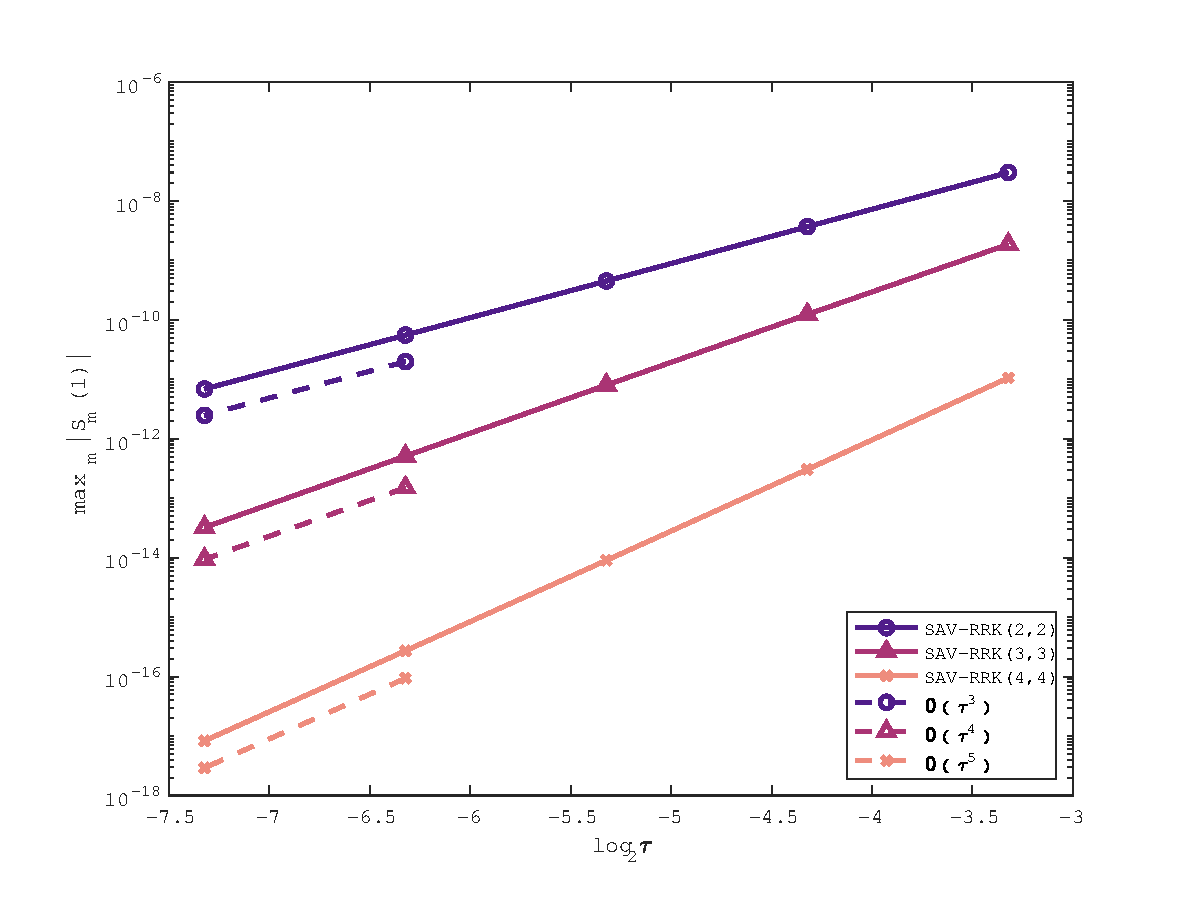
\includegraphics[width=0.5\textwidth]{./figures/exp1_s.eps}
% 	%\centerline{($a$) Temporal accuracy with $N=128.$}
% 	}\caption{松弛(RT)方法的 $\max _m\left|\gamma_m-1\right|$ 和 $\max_m\left|S_m(1)\right|$ (例 \ref{ex:1})} 
% 	\label{fig:1}
% 	\end{center}
% 	\end{figure}
  
%     此外,我们采用 $RK(4,4)$ 方法,计算不同 $\alpha$ 下的 $L^{\infty}$-范数误差.图 \ref{fig:2} 显示了解的误差及其在 $L^{\infty}$-范数下的收敛阶数,结果证实了 SAV-IDT 方案和 SAV-RRK 方案在时间方向上都具有四阶收敛性.我们在图 \ref{fig:3} 中描绘了不同 $N$ 和 $\tau=0.01$ 的方案的空间误差,结果显示出所提出的方案的空间误差非常小,几乎可以忽略不计,而误差主要由时间离散化误差所主导.这证实了对于充分光滑的问题,傅里叶伪谱方法在空间上是任意阶的.
%     \begin{figure}[H]
% 		\begin{center}
% 		\subfigure[$N=32 $(IDT)]{ \centering
% 		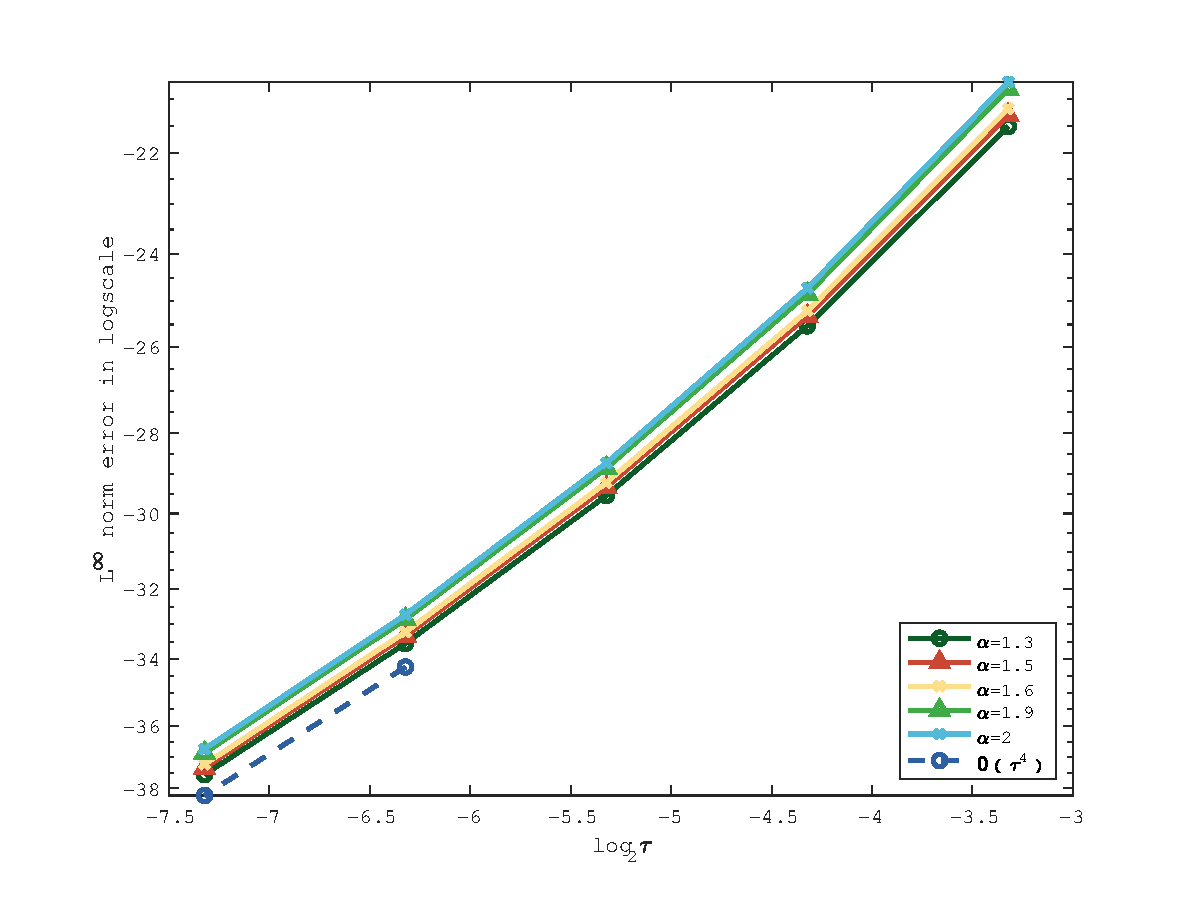
\includegraphics[width=0.5\textwidth]{./figures/exp1_RT_order_t.eps}
% 		%\centerline{($b$) Spatial accuracy with $\tau = 10^{-3}.$}
% 		}\subfigure[$N=32 $(RT)]{ \centering
% 		\includegraphics[width=0.5\textwidth]{./figures/exp1_IDT_order_t.eps}
% 		%\centerline{($a$) Temporal accuracy with $N=128.$}
% 		}\caption{不同 $\alpha$ 下 IDT 和 RT 的收敛阶数. (例 \ref{ex:1})} 
% 		\label{fig:2}
% 		\end{center}
% 		\end{figure}
% 	\begin{figure}[H]
% 		\begin{center}
% 		\subfigure[$\tau=0.01 $(IDT)]{ \centering
% 		\includegraphics[width=0.5\textwidth]{./figures/exp1_RT_order_s.eps}
% 		%\centerline{($b$) Spatial accuracy with $\tau = 10^{-3}.$}
% 		}\subfigure[$\tau=0.01 $(RT)]{ \centering
% 		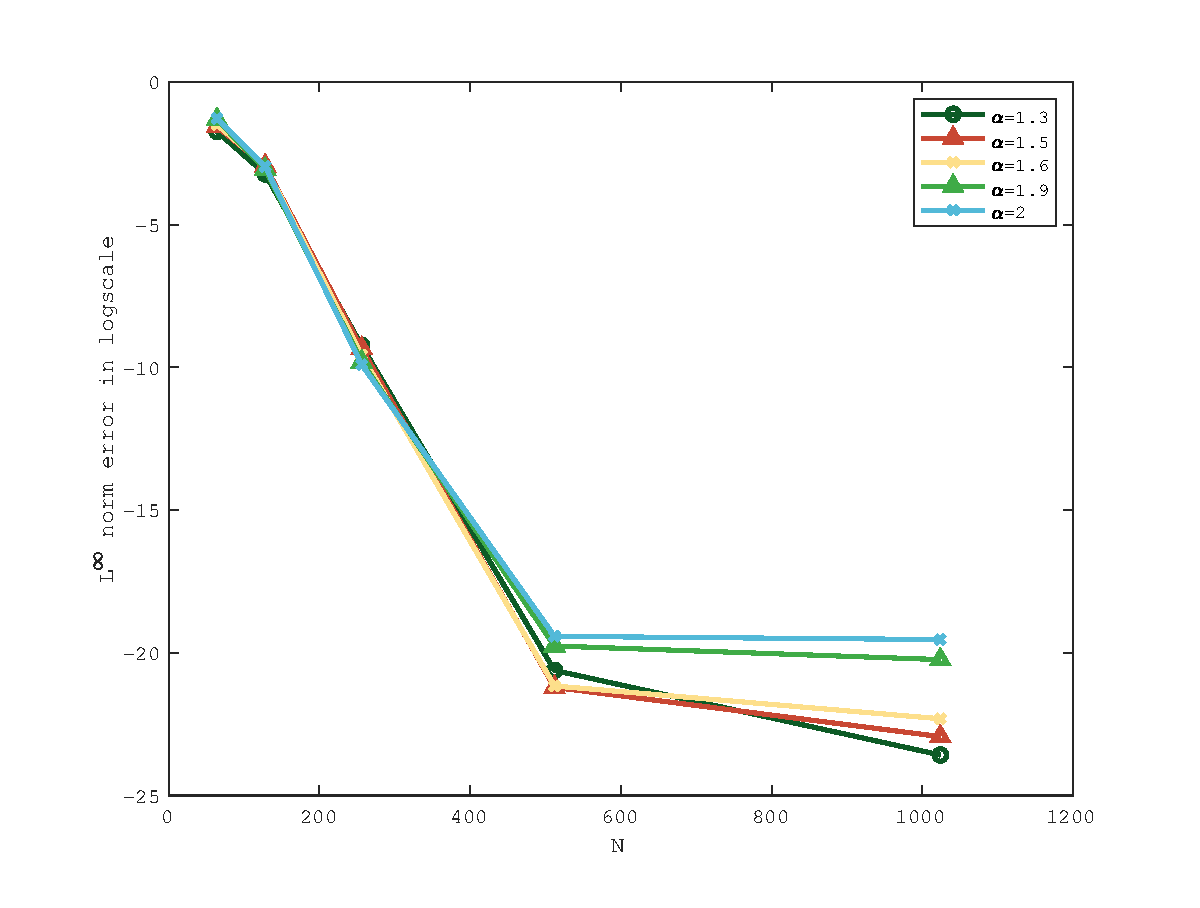
\includegraphics[width=0.5\textwidth]{./figures/exp1_IDT_order_s.eps}
% 		%\centerline{($a$) Temporal accuracy with $N=128.$}
% 		}\caption{不同 $\alpha$ 下 IDT 和 RT 的收敛阶数. (例 \ref{ex:1})} 
% 		\label{fig:3}
% 		\end{center}
% 		\end{figure}
% 		我们还进行了一次长时间模拟,直到 $T=1000$,并在图 \ref{fig:4} 中以不同的 $\alpha$ 绘制了 SAV-RRK(4,4) 方案的相对能量.结果表明,所提出的方案可以在离散场景中完全保持能量,并且其保持效果明显优于 SAV 方案和三级线性隐式差分方案.
%         \begin{figure}[H]
% 		\begin{center}
% 		\subfigure[$\alpha=1.3$]{ \centering
% 		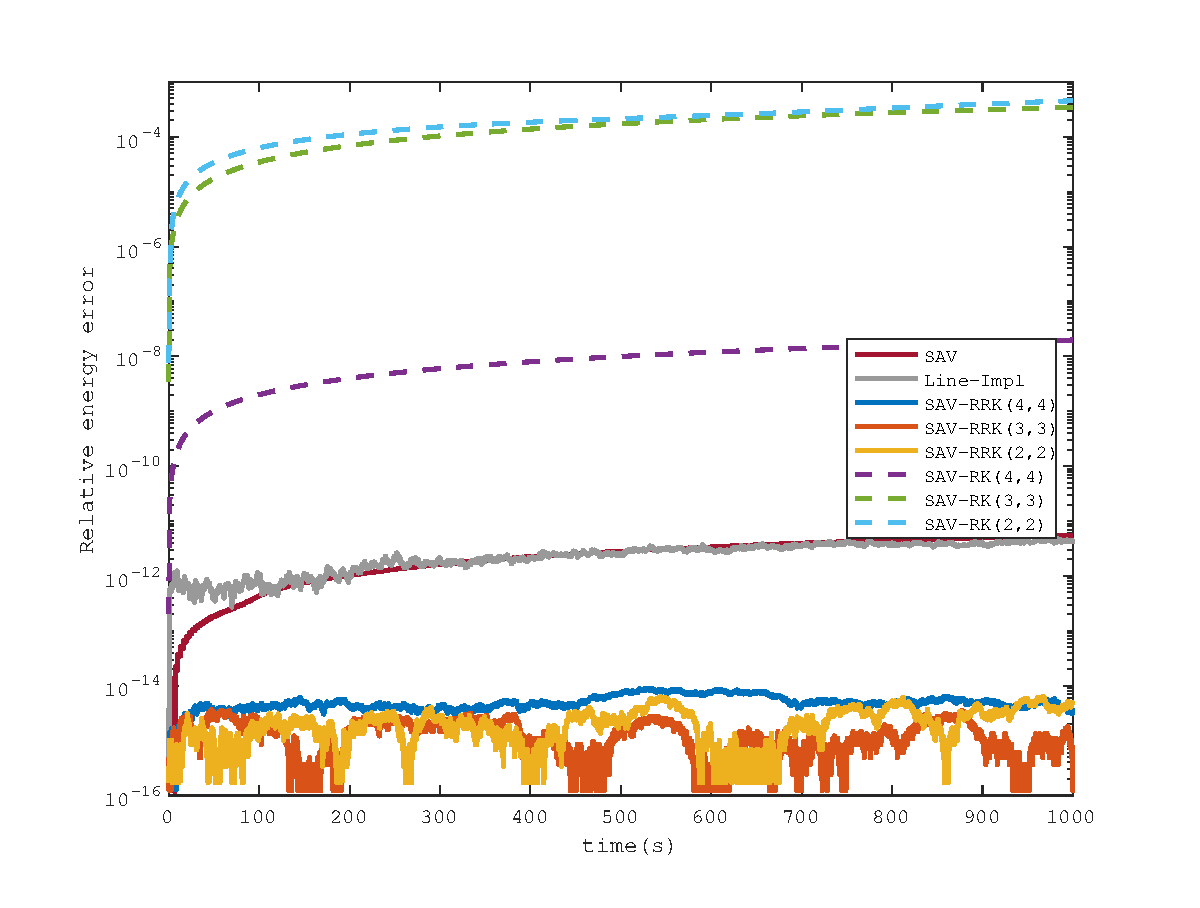
\includegraphics[width=0.5\textwidth]{./figures/exp1_energy3.eps}
% 		%\centerline{($b$) Spatial accuracy with $\tau = 10^{-3}.$}
% 		}\subfigure[$\alpha=1.6$]{ \centering
% 		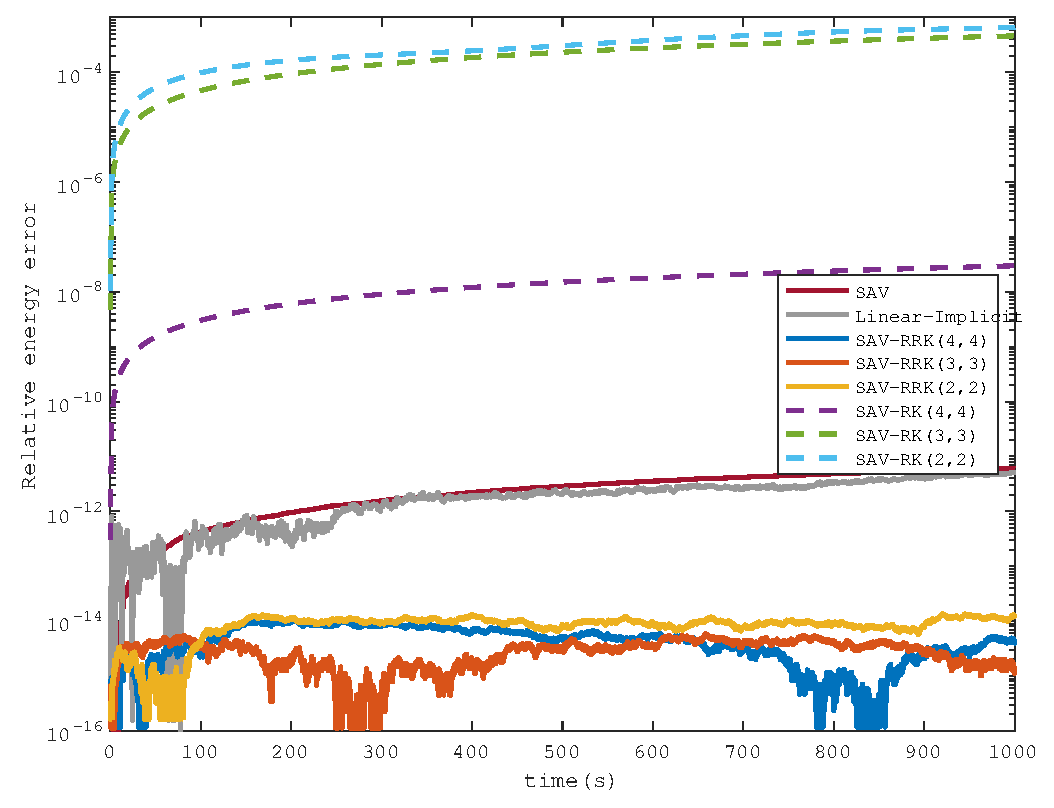
\includegraphics[width=0.5\textwidth]{./figures/exp1_energy6.eps}
% 		%\centerline{($a$) Temporal accuracy with $N=128.$}
% 		}\\
% 		\subfigure[$\alpha=1.9$]{ \centering
% 		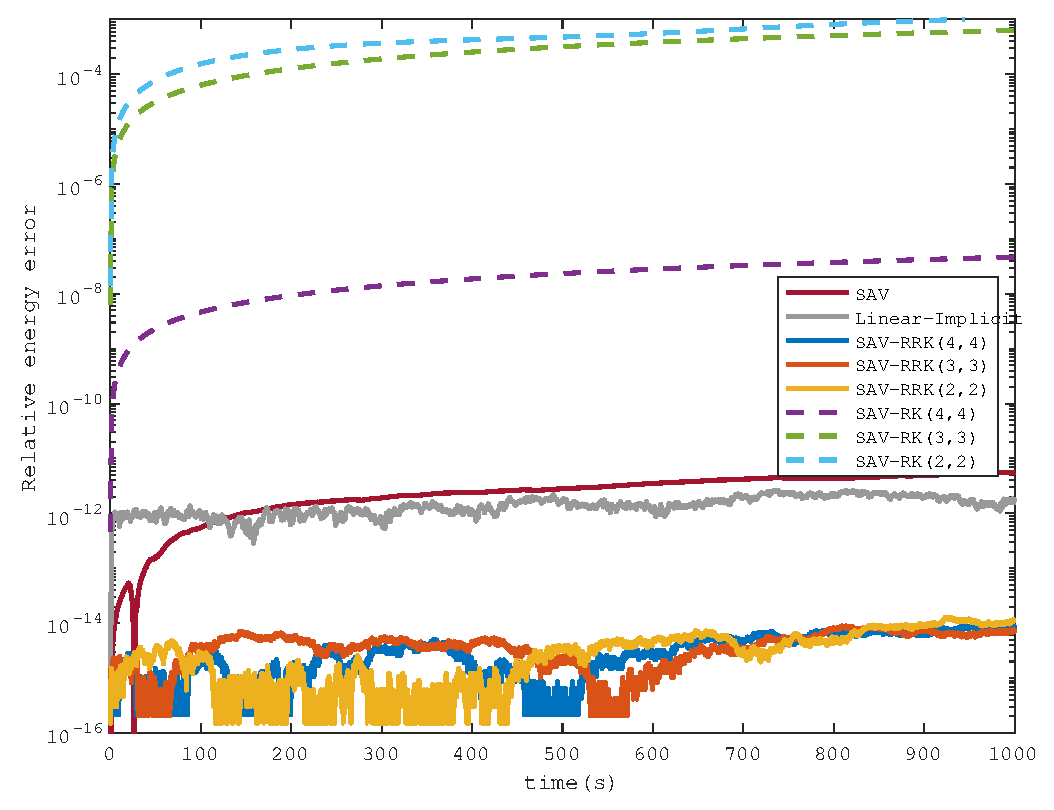
\includegraphics[width=0.5\textwidth]{./figures/exp1_energy9.eps}
% 		%\centerline{($b$) Spatial accuracy with $\tau = 10^{-3}.$}
% 		}\subfigure[$\alpha=2$]{ \centering
% 		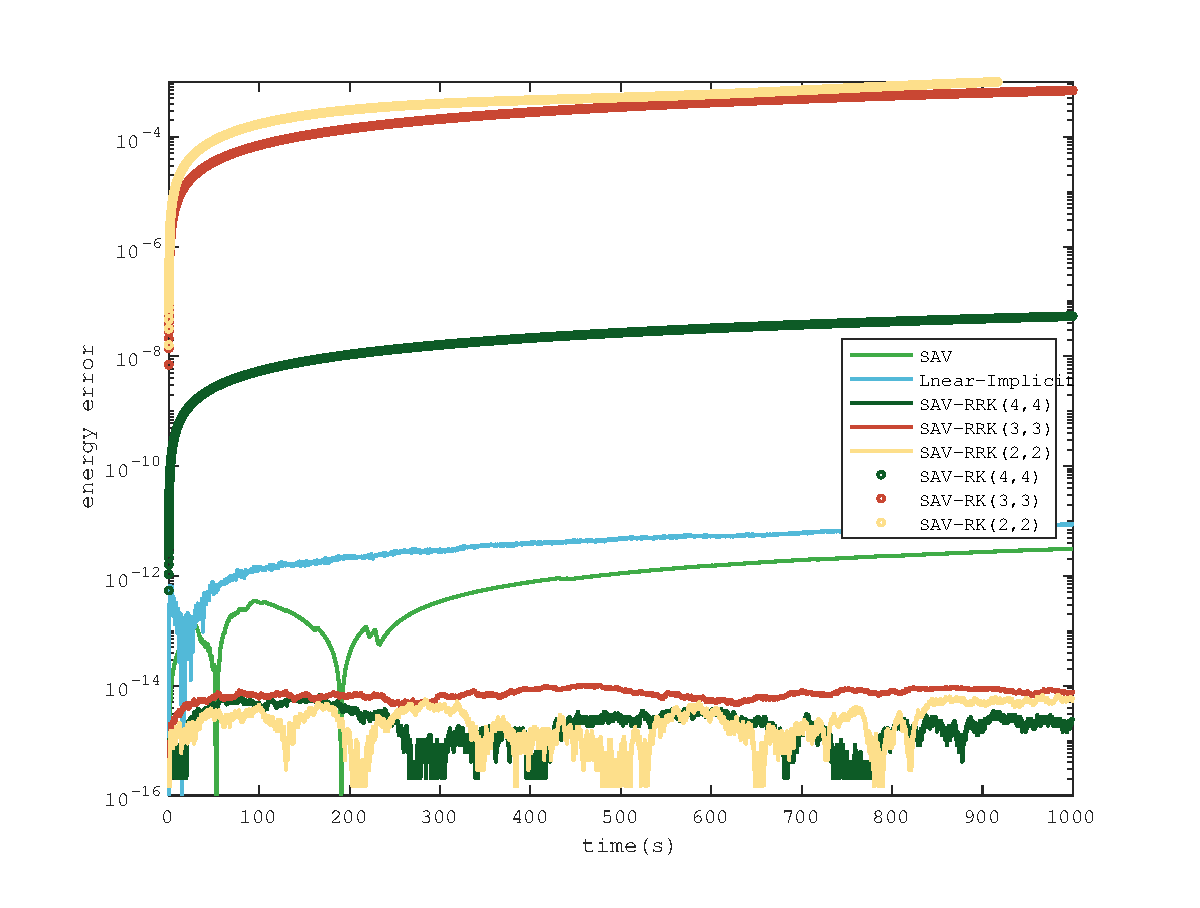
\includegraphics[width=0.5\textwidth]{./figures/exp1_energy2.eps}
% 		%\centerline{($a$) Temporal accuracy with $N=128.$}
% 		}\caption{ 当 $N=32$,$\tau=0.01$ 时,不同 $\alpha$ 下能量的相对误差.(例 \ref{ex:1})} 
% 		\label{fig:4}
% 		\end{center}
% 		\end{figure}

% \begin{example}\label{ex:2}
%     现在我们考虑带有初值的二维 NFSWEs \eqref{eq:s1}:
% \begin{equation}
% u(x, y, 0)=\operatorname{sech}\left(x^2+y^2\right), u_t(x, y, 0)=\sin (x+y) \operatorname{sech}\left(-2\left(x^2+y^2\right)\right),(x, y, t) \in \Omega \times[0, T],
% \end{equation}
% 其中 $\Omega=[-5,5] \times[-5,5]$.
% \end{example}
